% ===================== CHAPITRE 4 : CONCEPTION DES INTERFACES UTILISATEUR =====================

\section*{Introduction}
Ce chapitre décrit la conception des interfaces selon une démarche centrée
utilisateur~: personas et parcours, architecture de l'information, wireframes,
charte graphique, puis maquettes et prototype interactif réalisés sous
\textbf{Figma}.

\section{Démarche et outils}
\label{sec:demarche-ux}
La conception suit un processus itératif~: \textbf{comprendre} (besoins,
existant), \textbf{définir} (personas, parcours), \textbf{structurer}
(arborescence, wireframes), \textbf{maquetter} (charte, maquettes haute
fidélité), \textbf{prototyper} (enchaînement des écrans). L'outil retenu est
\textbf{Figma}, pour le travail collaboratif, la bibliothèque de composants
réutilisables et le mode prototype.

\section{Personas et parcours}
\label{sec:personas}

\begin{table}[H]
\centering
\renewcommand{\arraystretch}{1.25}
\begin{tabularx}{\linewidth}{>{\bfseries}p{3cm} X}
\toprule
Persona & Besoin principal \\
\midrule
Amine, 29 ans, locataire & Trouver un appartement proche de son travail~; usage mobile~; carte + filtres budget/quartier. \\
Sonia, 41 ans, propriétaire & Publier facilement sa villa~; positionner précisément le bien~; gérer les photos. \\
Karim, 35 ans, agent & Saisie rapide de nombreuses annonces~; espace dédié et tableau de bord. \\
Leïla, administratrice & File de modération claire~; vérification de la localisation~; motifs de refus normalisés. \\
\bottomrule
\end{tabularx}
\caption{Personas}
\label{tab:personas}
\end{table}

\begin{figure}[H]
  \centering
  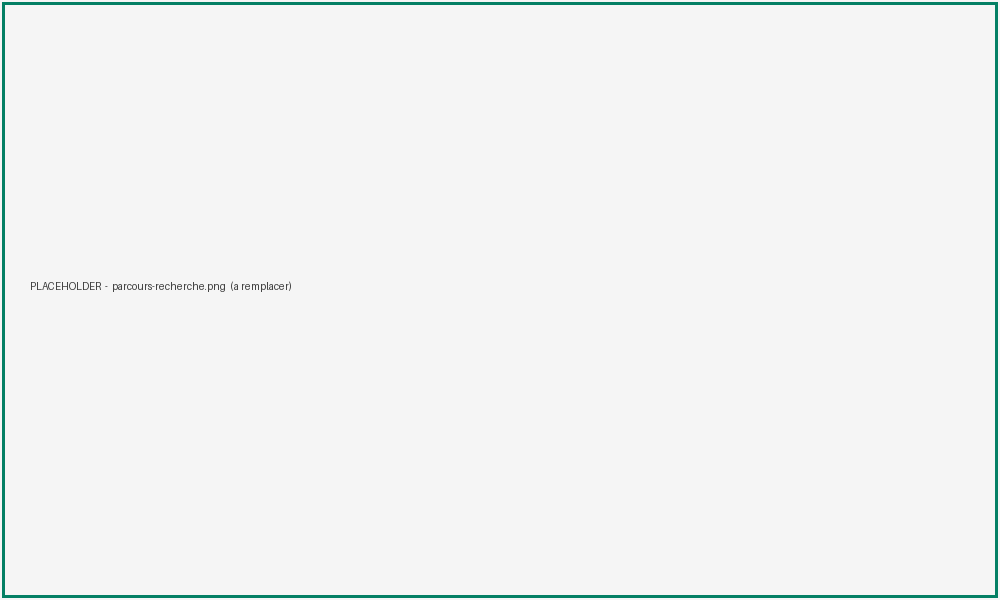
\includegraphics[width=0.9\linewidth]{images/parcours-recherche.png} % À FOURNIR (Figma)
  \caption{Parcours utilisateur « rechercher et contacter »}
  \label{fig:parcours-recherche}
\end{figure}
\noindent Étapes~: accueil $\rightarrow$ saisie d'un lieu ou géolocalisation
$\rightarrow$ carte + liste $\rightarrow$ affinage des filtres $\rightarrow$
fiche détaillée $\rightarrow$ favori / comparaison $\rightarrow$ contact.

\section{Architecture de l'information}
\label{sec:arbo}

\begin{figure}[H]
  \centering
  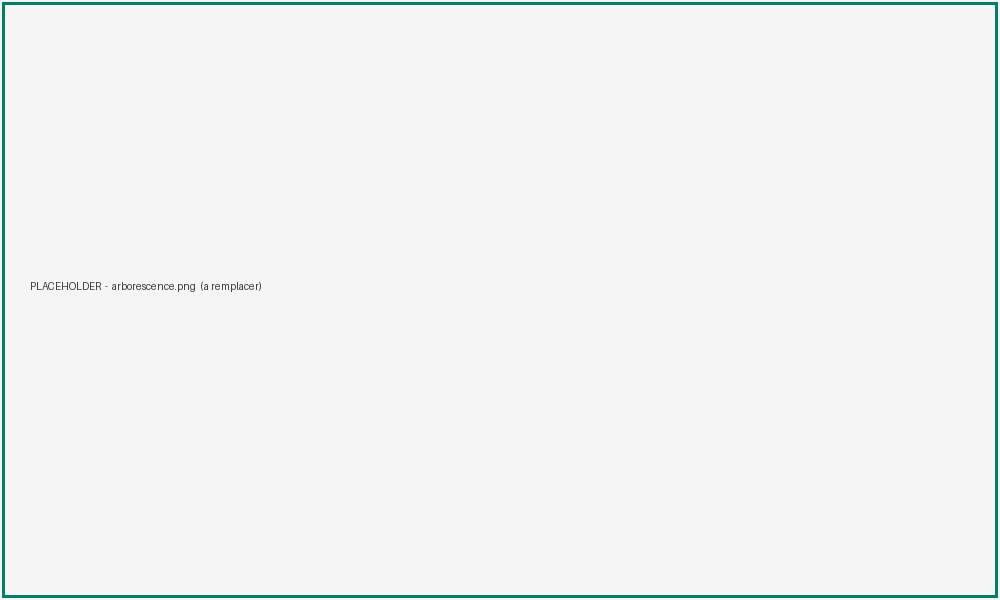
\includegraphics[width=0.92\linewidth]{images/arborescence.png} % À FOURNIR (Figma)
  \caption{Arborescence (plan de site)}
  \label{fig:arborescence}
\end{figure}

\begin{table}[H]
\centering
\renewcommand{\arraystretch}{1.2}
\begin{tabularx}{\linewidth}{>{\bfseries}p{3.2cm} X}
\toprule
Zone & Écrans \\
\midrule
Public        & Accueil, Recherche (liste), Recherche sur carte, Détail d'une annonce, Comparateur, Contenus (À propos, FAQ, Contact). \\
Compte        & Connexion, Inscription, Mot de passe oublié, Mon compte, Mes favoris, Mes recherches. \\
Publication   & Assistant « Créer une annonce » (multi-étapes), Modifier une annonce. \\
Professionnel & Espace agence (portefeuille, agents, tableau de bord). \\
Administration & Tableau de bord admin, modération des annonces, gestion des comptes. \\
\bottomrule
\end{tabularx}
\caption{Regroupement des écrans}
\label{tab:pages}
\end{table}

\noindent La navigation repose sur une barre persistante (logo, recherche,
« Publier », compte), une bascule \textbf{Liste $\leftrightarrow$ Carte} toujours
accessible, et un menu utilisateur contextuel selon le rôle.

\section{Wireframes (basse fidélité)}
\label{sec:wireframes}

\begin{figure}[H]
  \centering
  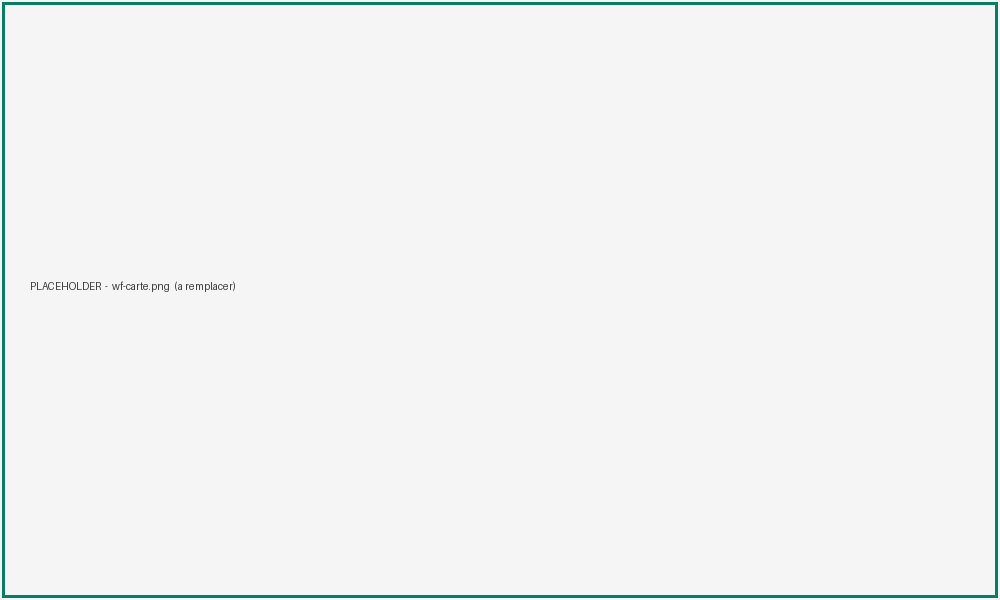
\includegraphics[width=0.9\linewidth]{images/wf-carte.png} % À FOURNIR (Figma)
  \caption{Wireframe : recherche sur carte}
  \label{fig:wf-carte}
\end{figure}
\noindent Colonne de filtres repliable, carte plein écran avec marqueurs
regroupés, panneau de résultats synchronisé avec l'emprise (survol croisé
carte $\leftrightarrow$ liste).

\begin{figure}[H]
  \centering
  
\includegraphics[width=0.9\linewidth]{images/wf-detail.png} % À FOURNIR (Figma)
  \caption{Wireframe : détail d'une annonce}
  \label{fig:wf-detail}
\end{figure}
\noindent Blocs~: galerie photos, titre + prix + localisation, caractéristiques,
description, \textbf{carte de situation}, équipements, bloc contact, biens
similaires.

\begin{figure}[H]
  \centering
  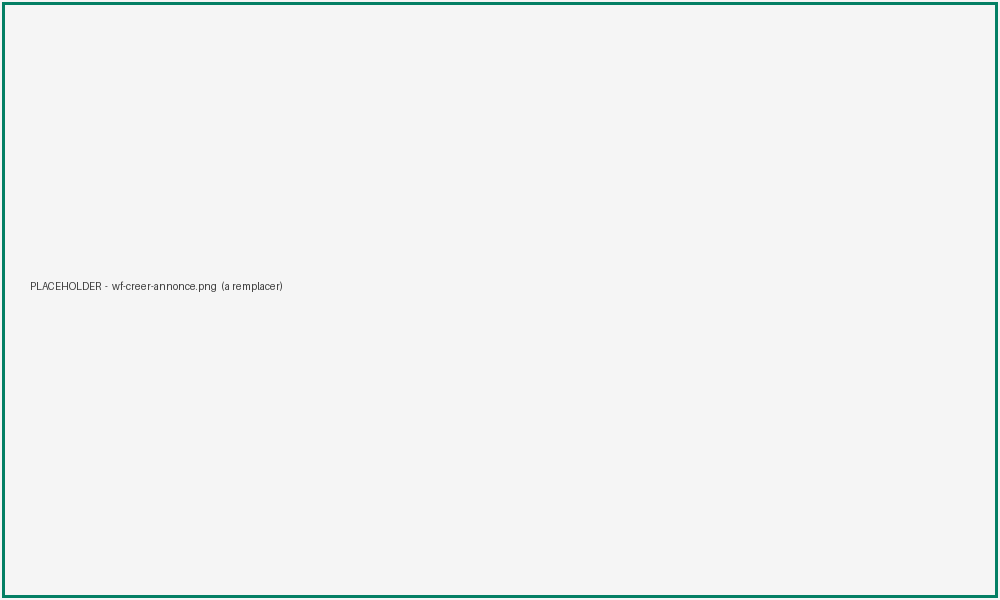
\includegraphics[width=0.9\linewidth]{images/wf-creer-annonce.png} % À FOURNIR (Figma)
  \caption{Wireframe : assistant « Créer une annonce »}
  \label{fig:wf-creer}
\end{figure}
\noindent Étapes~: (1) catégorie et type~; (2) caractéristiques~;
(3) \textbf{localisation} (référentiel + placement sur carte + géocodage
inverse)~; (4) photos (glisser-déposer)~; (5) prix et options~;
(6) récapitulatif et soumission~; une barre de progression indique l'étape.

\begin{figure}[H]
  \centering
  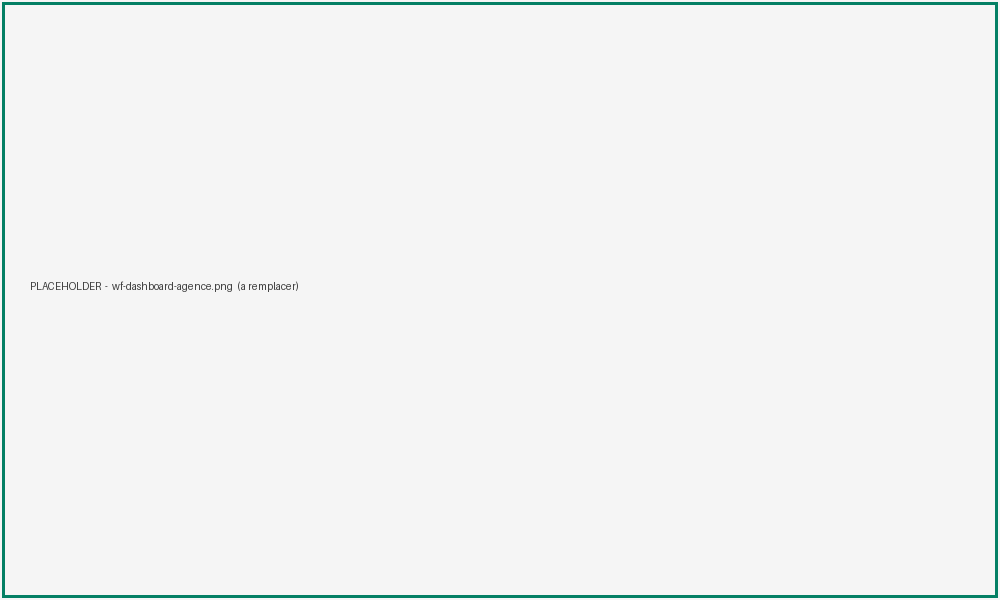
\includegraphics[width=0.9\linewidth]{images/wf-dashboard-agence.png} % À FOURNIR (Figma)
  \caption{Wireframe : tableau de bord agence}
  \label{fig:wf-dashboard}
\end{figure}

\section{Charte graphique}
\label{sec:charte}

\begin{table}[H]
\centering
\renewcommand{\arraystretch}{1.25}
\begin{tabularx}{\linewidth}{>{\bfseries}p{3cm} p{3cm} X}
\toprule
Rôle & Code (exemple) & Usage \\
\midrule
Primaire   & \texttt{\#047F64} & Actions principales, liens, marqueurs actifs. \\
Secondaire & \texttt{\#0077B6} & Accents, éléments d'information. \\
Accent     & \texttt{\#ED6E0A} & Mises en avant, badges. \\
Fond neutre & \texttt{\#F5F5F5} & Arrière-plans de sections. \\
Texte      & \texttt{\#1F2937} & Corps de texte. \\
Succès / Erreur & \texttt{\#16A34A} / \texttt{\#DC2626} & États de validation. \\
\bottomrule
\end{tabularx}
\caption{Palette de couleurs (à valider avec la charte de l'organisme)}
\label{tab:palette}
\end{table}

\noindent \textbf{Typographie}~: police sans empattement lisible à l'écran
(ex.~\emph{Inter} / \emph{Poppins})~; hiérarchie H1--H3, corps 16~px, légendes
13~px~; interlignage 1,5.
\textbf{Composants Figma}~: boutons, champs, listes déroulantes dépendantes
(gouvernorat $\rightarrow$ délégation $\rightarrow$ localité), cartes de bien,
marqueurs et \emph{popups}, fenêtres modales, \emph{toasts}, barre de
progression, pagination.
\textbf{Rendu cartographique}~: marqueur standard, marqueur mis en avant,
marqueur sélectionné~; pastille numérotée pour le regroupement~; \emph{popup} au
clic (photo, prix, titre, lien vers la fiche).

\section{Maquettes haute fidélité et prototype}
\label{sec:maquettes}

\begin{figure}[H]
  \centering
  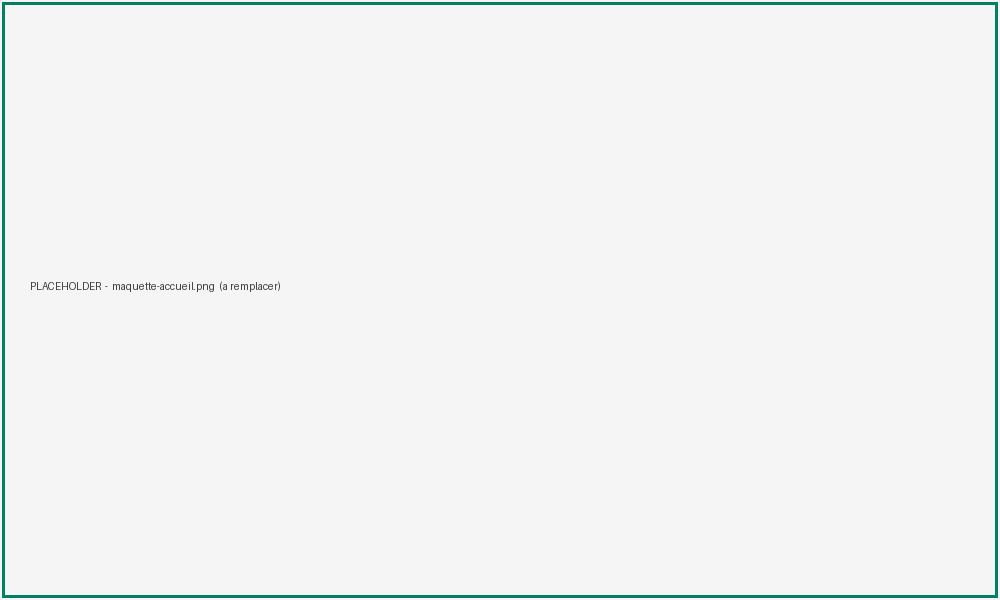
\includegraphics[width=0.9\linewidth]{images/maquette-accueil.png} % À FOURNIR (Figma)
  \caption{Maquette haute fidélité : page d'accueil}
  \label{fig:maquette-accueil}
\end{figure}

\begin{figure}[H]
  \centering
  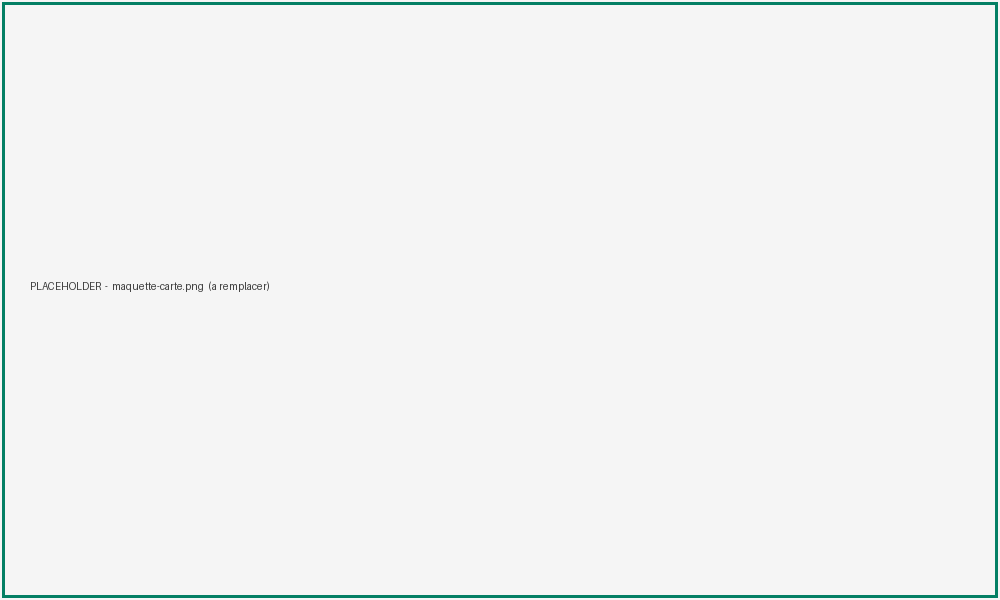
\includegraphics[width=0.9\linewidth]{images/maquette-carte.png} % À FOURNIR (Figma)
  \caption{Maquette haute fidélité : recherche sur carte}
  \label{fig:maquette-carte}
\end{figure}

\begin{figure}[H]
  \centering
  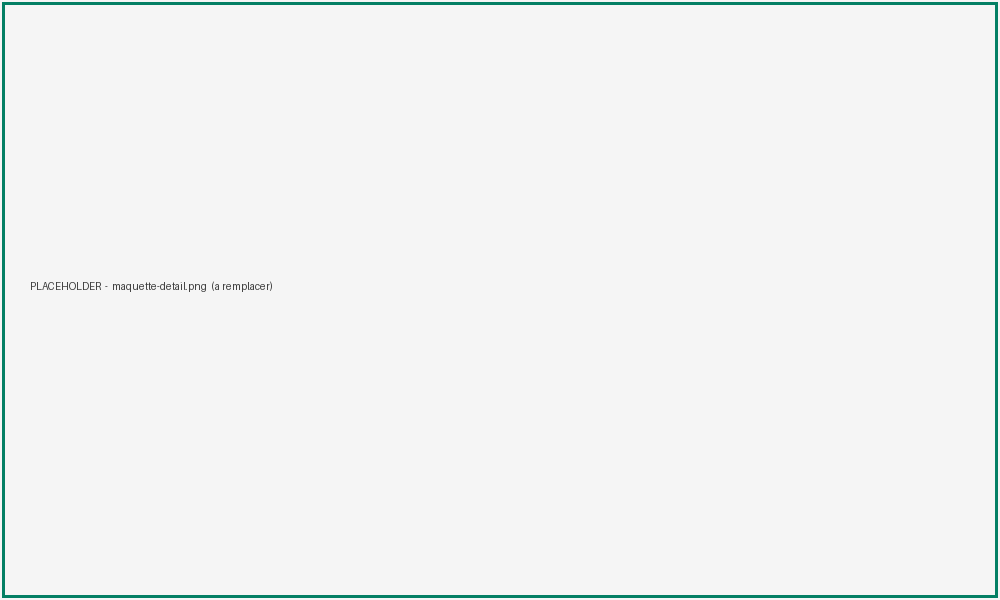
\includegraphics[width=0.9\linewidth]{images/maquette-detail.png} % À FOURNIR (Figma)
  \caption{Maquette haute fidélité : détail d'une annonce}
  \label{fig:maquette-detail}
\end{figure}

\noindent Les écrans sont reliés dans le \textbf{mode prototype de Figma} pour
simuler les parcours principaux (recherche, publication, modération) et valider
l'enchaînement des interactions avant tout développement. Lien du prototype~:
[\ldots].

\section{Ergonomie et accessibilité}
\label{sec:accessibilite}
\begin{itemize}[label=\textbullet,itemsep=1pt]
  \item respect des heuristiques de Nielsen (retour d'information, prévention des
        erreurs, cohérence, contrôle utilisateur)~;
  \item conformité visée \textbf{WCAG 2.1 niveau AA}~: contrastes suffisants,
        navigation clavier, libellés de formulaire explicites, textes
        alternatifs, cibles tactiles $\geq$ 44~px~;
  \item conception \textbf{responsive} (points de rupture indicatifs 360, 768,
        1024, 1280~px)~; filtres et liste en tiroirs sur mobile.
\end{itemize}

\section*{Conclusion}
La conception des interfaces est complète~: personas et parcours, arborescence,
wireframes, charte graphique, maquettes et prototype Figma. L'ensemble constitue
une base prête pour la phase de développement.
